%++++++++++++++++++++++++++++++++++++++++
% Don't modify this section unless you know what you're doing!
\documentclass[letterpaper,11pt]{article}
\usepackage{natbib}
\bibliographystyle{unsrtnat}
\usepackage{multicol}
\usepackage{lmodern}
\usepackage{blindtext}
% (2) specify encoding
\usepackage[T1]{fontenc}
\usepackage[utf8]{inputenc}
% (3) load symbol definitions
\usepackage{textcomp}
\usepackage{tabularx} % extra features for tabular environment
\usepackage{amsmath}  % improve math presentation
\usepackage{graphicx} % takes care of graphic including machinery
\usepackage[margin=1in,letterpaper]{geometry} % decreases margins
%\usepackage{cite} % takes care of citations
\usepackage[final]{hyperref} % adds hyper links inside the generated pdf file
\hypersetup{
	colorlinks=true,       % false: boxed links; true: colored links
	linkcolor=blue,        % color of internal links
	citecolor=blue,        % color of links to bibliography
	filecolor=magenta,     % color of file links
	urlcolor=blue         
}
%++++++++++++++++++++++++++++++++++++++++




\title{PREDICT COVID-19 WITH BEST MODEL\\ BASED ON SYMPTOM }
\author{%
Md Fahim Faez Abir$^{1}$ \\
2018-1-60-032\\
\\
Nazmus Sakib$^{2}$ \\ 
2018-1-60-104\\
\\
Md. Tanbin Hossain Himel$^{3}$ \\
2018-1-60-151\\
\\
Kamruzzaman Leeon$^{4}$ \\ 
2018-1-60-252\\
}
\setlength{\parskip}{2em}
\date{MAY 26, 2021}

\begin{document}
\maketitle


\setlength{\parindent}{0em}
\setlength{\parskip}{1em}

\section{Introduction}

Coronavirus disease (COVID-19) is a newly found coronavirus that causes an infectious illness. The majority of patients infected with the COVID-19 virus will have mild to moderate respiratory symptoms and will recover without needing any specific therapy. People over the age of 65 and infants, as well as those with underlying medical conditions such as cardiovascular disease, diabetes, chronic respiratory disease, and cancer, are at a higher risk of developing serious illness \cite{who_web1}. It was first detected in humans by scientists in 1965.  Later in 2019, COVID was found in Wuhan city, china and renamed as COVID-19. And now it has become a global pandemic all over the world \cite{web_md6}.\\
\\
Therefore, our problem is to find the best estimator model and find the dependency of the best estimator model so that, we can distinguish COVID-19 patient. We intended to do the project because at present COVID-19 test is time-consuming and costly. Therefore, it is convenient for a person if he can get a pre-result before final test.\\
\\
We have found some existing work on this problem. The motivation as well as the objective of these works are as same as ours but most of them have some lacking i.e. lack of real data-set, lack of authentic data set, complexity of the algorithms. We also found some image processing work on COVID-19 but seems less convenient at the present scenario in terms of cost \cite{Xray}. \\
\\
The necessity of the project on this topic is very important at this moment, because currently we are currently undergoing a pandemic situation. The only prevention of COVID-19 is available at this moment is to take care of the patient after identifying symptoms. Therefore, it is convenient for us if we can distinguish COVID patient as early as possible and take initiative for taking care of the patient.
\\
\section{Methodology}
Our first task was to collect real data of patients. After collecting several data-set we have to find relevant data-set, we preprocessed the data. After that, we analyze the importance of the features. When we finalize the features, we divide the data-set into 3 types and create five model i.e. Random Forest, Logistic Regression, Neural Network, Decision Tree & Naïve Bayes. Finally, we train our models with the data-sets and conclude our result. \\

\date{}

\graphicspath{Images/}
\begin{figure}[htp]
    \centering
    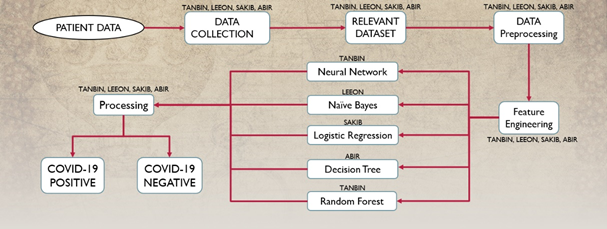
\includegraphics[width=15cm\textwidth]{image1.png}
    \caption{our methodology}
        \label{fig:F1}
\end{figure}

\section{Implement}

\subsection{Data collection}

\noindent
We have collected our data from Kaggle. We have found several data-sets on COVID-19. But we select a data-set titled “COVID-19 symptom checker” \cite{symCheck}. Because the data provider assures us that it was originally collected from WHO without any manipulation. Therefore it can be assumed that, it is an authentic data-set with real values.\\
Our dataset has 22 attributes i.e. 'Fever','Tiredness', 'Dry-Cough', 'Difficulty-in-Breathing', 'Sore-Throat', 'None{\_}Sympton', 'Pains', 'Nasal-Congestion', 'Runny-Nose', 'Diarrhea', 'None{\_}Experiencing', 'Age{\_}0-9', 'Age{\_}10-19', 'Age{\_}20-24', 'Age{\_}25-59', 'Age{\_}60+', 'Gender{\_}Female', 'Gender{\_}Male', 'Gender{\_}Transgender', 'Contact{\_}Dont-Know', 'Contact{\_}No', 'Contact{\_}Yes’. Almost 316800 peoples data have been collected here. From the dataset we can observe that, gender is divided into 3 sub-columns, age is divided into 5 sub-columns. Also, we found that all the columns are related to COVID-19. We also notice that, the deciding factor of the dataset is divided into four sub-columns i.e Severity{\_}Mild, Severity{\_}Moderate, Severity{\_}None, Severity{\_}Severe.


\subsection{Data Processing}

\noindent
Our data was not fully organized before. Here we observe that our data-set has a country column which has 10 different values. Therefore, we convert it into 10 sub-columns i.e. 'Country{\_}China', 'Country{\_}France', 'Country{\_}Germany','Country{\_}Iran','Country{\_}Italy', 'Country{\_}Other', 'Country{\_} Other-EUR', 'Country{\_}Republic of Korean', 'Country{\_}Spain' & 'Country{\_}UAE'.
Since our deciding factor is divided into 4 sub-columns, we decided to make three types of data-sets here based on the deciding factor. 





\begin{table}[ht]
\begin{center}
\caption{Every table needs a caption.}
\label{table1} 
\begin{tabular}{cccc} 
\hline
\multicolumn{1}{c}{Value} & \multicolumn{1}{c}{Type-01} & \multicolumn{1}{c}{Type-02}& \multicolumn{1}{c}{Type-03}\\
\hline
None     &   0 &   0 &   0 \\
mild     &   1 &   0 &   1 \\
moderate &   1 &   1 &   2 \\
severe   &   1 &   1 &   3 \\
\hline
\end{tabular}
\end{center}
\end{table}

\begin{itemize}
  \item \textbf{Type 1:}
  Here, we decided to convert the deciding factor into binary values 0 & 1 where 1 means ‘yes’ and 0 means ‘no’. If we ignore the level of severity, ‘Mild’, ‘moderate’ & ‘severe’ means that the person actually has COVID-19. Therefore, we convert these three values into ‘yes’. On the other hand, None means the person does not have COVID-19. Therefore, we convert it into ‘no’.

  \item \textbf{Type 2:}
  Here also, we decided to convert the deciding factor into binary values 0 & 1 where 1 means ‘yes’ and 0 means ‘no’. ‘None’ & ‘Mild’, means that the person does not have COVID-19 or has a few symptoms of COVID-19. Therefore, we assume it as negative and convert these two values into ‘no’. On the other hand, ‘moderate’ & ‘severe’ means the person has symptoms of COVID-19 but the severity of the symptoms is higher than ‘None’ and ‘Mild’. Therefore, we assume it as positive and convert these two values into ‘yes’.

  \item \textbf{Type 3:} 
  Here we divided the deciding factor according to its level of severity. The more the values the higher the level of severity. Therefore, ‘none’ is converted into 0, ‘mild’ is 1, ‘moderate’ is 2 and severe is 3. 

\end{itemize}
With these three types of data, we decided to train and test our model separately and compare them. 


\section{Model Development}
We have worked with five models i.e. Random forest, Logistic Regression, Decision Tree, Gaussian Naive Bayes & Neural networks so that we can compare the accuracy between the models and find the best estimator.
\begin{itemize}
  \item \textbf{Random forest:}A random forest is a meta estimator that uses averaging to improve projected accuracy and control over-fitting by fitting several decision tree classifiers to different sub-samples of the dataset. The sub-sample size is controlled by the max samples parameter if bootstrap=True (default); otherwise, the whole dataset is used to generate each tree \cite{random_forest3}.
  
  \item \textbf{Logistic Regression:}Logistic regression is a classification model, not a regression model, despite its name. In the literature, logistic regression is also known as logit regression, maximum-entropy classification (MaxEnt), or the log-linear classifier. In this approach, a logistic function is employed to characterize the likelihood of the likely outcomes of a single experiment \cite{lr4}.
  
  \item \textbf{Decision Tree:}
  The decision Tree is a supervised learning method for classification and    regression that is non-parametric. The goal is to learn basic decision rules from data attributes and build a model that predicts the value of a target variable. A piecewise constant approximation is a tree. The decision criteria become more complex as the tree goes deeper and the model becomes more accurate \cite{dt2}. The necessary equation to calculate decision tree:
  
 \date{}

\graphicspath{Images/}
\begin{figure}[htp]
    \centering
    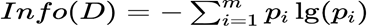
\includegraphics[width=4cm\textwidth]{DT1.png}\\
    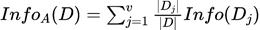
\includegraphics[width=4cm\textwidth]{DT2.png}\\
    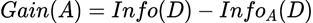
\includegraphics[width=4cm\textwidth]{DT3.png}\\
\end{figure}
  
  \item \textbf{Gaussian Naive Bayes:}Naive Bayes approaches are supervised learning methods based on Bayes' theorem with the "naive" assumption of conditional independence between every pair of features given the class variable value. The Gaussian Naive Bayes approach is used in GaussianNB, a classification tool\cite{nb5}. The features' probability is considered to be Gaussian:
  \date{}

\graphicspath{Images/}
\begin{figure}[htp]
    \centering
    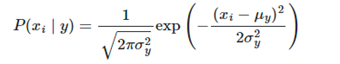
\includegraphics[width=6cm\textwidth]{GNB.png}\\
   
\end{figure}
  \item \textbf{Neural Network:}
  A neural network is a reliable method for forecasting real, discrete, or vector data. It's based on the biological learning system and can tackle biological as well as non-biological challenges.\\
 \date{}
\graphicspath{Images/}
\begin{figure}[htp]
    \centering
    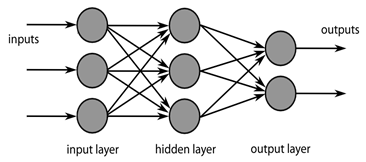
\includegraphics[width=6cm\textwidth]{NN.png}\\
\end{figure}
  \\Nodes, edges, edge widgets, and bias are the representative elements.


\end{itemize}


\section{Result}
\\The results of the models is given below:
\begin{table}
\begin{center}
%\caption{The results of the models is given below:}
\label{table1} 
\begin{tabular}{ccccccc} 
\hline
\multicolumn{1}{c}{Value} & \multicolumn{2}{c}{Type-01} & \multicolumn{2}{c}{Type-02}& \multicolumn{1}{c}{Type-03}\\
\hline
Name & 	accuracy &	F1 accuracy &	accuracy &	F1 accuracy &	accuracy &	F1 accuracy\\
Random Forest &	68.96\%	& 40.81\%	& 16.35\% &	16.35\% &	0.21\% &	0.21\% \\
logistic Regression &	74.91\%	& 53.33\% &	49.45\%	& 49.45\% &	24.05\%	& 23.87\%\\
Decision Tree &	53.33\% &	34.83\% &	16.35\%	& 14.95\% &	0.21\% &	0.15\% \\
Gaussian Naive Bayes &	74.91\% &	42.83\% &	49.58\%	& 49.33\% &	24.29\% &	24.06\%\\
Neural Network &	74.91\% &	42.83\%	& 42.83\% &	43.41\% &	23.53\%	& 15.22\%\\
\hline
\end{tabular}
\end{center}
\end{table}

Here we observe that the accuracy level depends on the classification of the deciding factor.
The accuracy of the Type-03 dataset is ranging from 0 to 25\%, the Type-02 dataset is ranging from 16-50\%, and the Type-01 is ranging from 53-74\%.
After observing the ROC curve we can see that, false positive rate is much more higher than true positive rate. As a reason we can observe that, the value of the dataset is not sufficient since COVID-19 is a new case for the world. As well as there is a lot of anomaly in the dataset. For that reason, the model is confused to truly identify positive cases and ROC curve value is negative.
We can also conclude that the accuracy is dependent on the model. Here we can see that Random Forest & Decision Tree has less accuracy in every type of dataset. On the other hand, Logistic Regression, Naive Bayes, and Neural Network have the same type of higher accuracy.
In term of f1 score, we can see that f1 scores value is higher in type-02 dataset compared to type-01 dataset.
From the above discussion we can conclude that, Logistic Regression is work well among all types of dataset since its accuracy and f1 accuracy are higher than other models. Therefore our best estimator model is Logistic Regression for distinguish COVID-19 patient.
\\
\\
\\
\graphicspath{Images/}
\begin{figure}[htp]
    \centering
    \begin{minipage}[b]{.48\textwidth}
        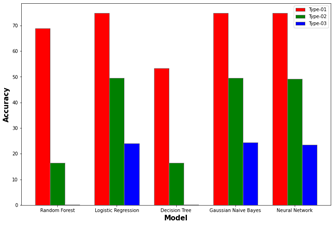
\includegraphics[width=8cm\textwidth]{Accuracy.png}
        \caption{Accuracy}
        \label{fig:Accuracy}
    \end{minipage}
    \begin{minipage}[b]{.48\textwidth}
        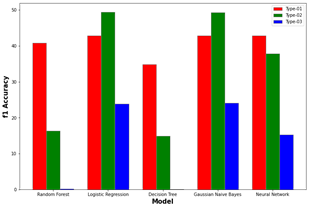
\includegraphics[width=8cm\textwidth]{f1.png}
        \caption{F1}
        \label{fig:F1}
    \end{minipage}
\end{figure}
\\
\begin{figure}[htp]
    \centering
    \begin{minipage}[b]{.40\textwidth}
        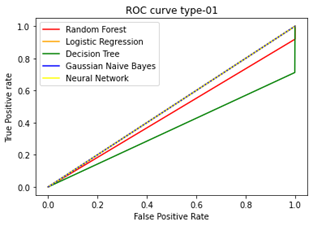
\includegraphics[width=8cm\textwidth]{ROC1.png}
        \caption{ROC curve type-01}
        \label{fig:ROC1}
    \end{minipage}
    \begin{minipage}[b]{.40\textwidth}
        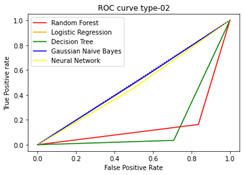
\includegraphics[width=8cm\textwidth]{roc2.png}
        \caption{ROC curve type-02}
        \label{fig:ROC2}
    \end{minipage}
\end{figure}



\\

\section{Conclusions}
\subsection{challenges}
The first challenges we have faced to collect the authentic dataset with real values. There are several datasets available but either they are found not authentic or the dataset is manipulated. Since we are trying to estimate the best model with real values, we must avoid these datasets. Another challenge was to find the higher accuracy of the best estimators. Since COVID-19 is a new disease we do not have enough data to take the accuracy at its peak.  \\
\\
\subsection{Limitations}
In the Type-3 dataset, we divided the deciding factor according to its level of severity. As a result, It has 4 values ranging from 0 to 3. As a result, its accuracy is too less than our expectation and we are not able to make any perfect model using it.\\
\\
\subsection{Future direction}
We have some learning from our project. Our first learning is to work with the project with sufficient amount of real values. Otherwise it is not possible for the model to predict the COVID-19 in real life scenario. Since, We found that Type-01 & Type-02 dataset has higher accuracy than Type-03 dataset, Therefore our recommendation is to classify the deciding factor into binary values. Also, we recommend to use dataset with having less anomaly so that the model can distinguish COVID-19 patient.\\ 
\\



\medskip
\begin{thebibliography}{99}

\bibitem{who_web1} 
World Health Organization: Coronavirus,
\\\texttt{https://www.who.int/health-topics/coronavirus\#tab=tab\_1}

\bibitem{web_md6} 
WebMD: Coronavirus History,
\\\texttt{https://www.webmd.com/lung/coronavirus-history}

\bibitem{random_forest3} 
scikit-learn: Random Forest Classifier,
\\\texttt{https://scikit-learn.org/stable/modules/generated/sklearn.ensemble.RandomForestClassifier.html}

\bibitem{lr4} 
scikit-learn: Logistic Regression,
\\\texttt{https://scikit-learn.org/stable/modules/linear\_model.html\#logistic-regression}

\bibitem{dt2} 
scikit-learn: Decision Trees,
\\\texttt{https://scikit-learn.org/stable/modules/tree.html}

\bibitem{nb5} 
scikit-learn: Gaussian Naive Bayes,
\\\texttt{https://scikit-learn.org/stable/modules/naive_bayes.html/#gaussian-naive-bayes}

\bibitem{Xray} 
Kaggle: COVID-19 X-ray image classification,
\\\texttt{https://www.kaggle.com/c/stat946winter2021}

\bibitem{symCheck} 
Kaggle: COVID-19 Symptoms Checker,
\\\texttt{https://www.kaggle.com/iamhungundji/covid19-symptoms-checker}

\end{thebibliography}








\end{document}
